% Research report, EPSRC DLA project S3.5-COM-Valentino (University of Sheffield).
% Format: IEEEtran conference, mirroring the ICRA template preamble (letterpaper, 10pt, helvet, cite).
% Build:  cd docs/proposal && latexmk -pdf report-full.tex   Check:  pdfinfo report-full.pdf  ->  Pages: 4 at most
% Compact report: every generated figure from README.md, no app screenshots, each figure beside its text in README order
% (13-page version: report-full-13p.tex).
% Structure: Abstract (from the literature in docs/paper) -> Introduction -> Method -> Results -> Conclusion.
% Numbers come only from README.md; citations only from docs/paper/ and
% research_notes/Neurosymbolic world models proposal/ (verified earlier).
\documentclass[letterpaper, 10pt, conference]{IEEEtran}
\IEEEoverridecommandlockouts
\usepackage{amsmath,amssymb}
\usepackage{graphicx}
\usepackage{booktabs}
\usepackage{array}
\usepackage{xcolor}
\usepackage{cite}
\usepackage{capt-of}
\usepackage[hidelinks]{hyperref}
\usepackage[scaled=0.92]{helvet}
\setlength{\textfloatsep}{8pt plus 2pt minus 2pt}
\setlength{\dbltextfloatsep}{8pt plus 2pt minus 2pt}
\setlength{\floatsep}{7pt plus 2pt minus 2pt}\setlength{\intextsep}{6pt plus 2pt minus 2pt}
\graphicspath{{../images/}}
\AtBeginDocument{\setlength{\abovedisplayskip}{2pt}\setlength{\belowdisplayskip}{2pt}}
\renewcommand{\topfraction}{0.9}\renewcommand{\dbltopfraction}{0.9}
\setcounter{dbltopnumber}{2}\renewcommand{\textfraction}{0.07}\renewcommand{\floatpagefraction}{0.9}

\newcommand{\applicant}{Ned Pham}   % <- check spelling, then rebuild
\newcommand{\demourl}{https://neural-symbolic-nlp.onrender.com/train-neural-symbolic}
\newcommand{\codeurl}{https://github.com/nhan03bit/neural_symbolic_nlp}

% Header box (as in the ICRA template): abstract and index terms left, Fig. 1 (core logic) right.
% The abstract summarises the literature in docs/paper, not the implementation.
\definecolor{absgray}{gray}{0.92}
\newcommand{\abstracttext}{Neural networks trained by next-word prediction are strong at perception, but keep no explicit link to the rules behind a decision. Sheth, Roy and Gaur argue that safety-critical AI needs knowledge set as guardrails during training, not after it, and sort neurosymbolic methods into \emph{lowering}, which compresses symbolic knowledge into the network, and \emph{lifting}, which maps neural outputs to symbols for reasoning. On the lowering side, the semantic loss of Xu et al.\ turns a logical constraint into a training term. Ahmed et al.\ extend it to autoregressive models, where the exact probability of a constraint is \#P-hard, and on GPT-2 pair it with word banning at decoding. A loss gives no test-time guarantee, and a mask leaves the model unchanged. This report asks what happens when one knowledge base drives both and a verifier lifts the output back to symbols, on a small transformer, and proposes the same split for neurosymbolic world models in robotic manipulation.}
\makeatletter
\let\old@maketitle\@maketitle
\renewcommand{\@maketitle}{\old@maketitle\vspace{-4pt}\setcounter{figure}{0}
\noindent\colorbox{absgray}{\begin{minipage}{\dimexpr\textwidth-2\fboxsep\relax}
\begin{minipage}[c]{0.445\linewidth}\sffamily\small\bfseries
\textit{Abstract}---\abstracttext\par\smallskip
\textit{Index Terms}---Neuro-symbolic AI, lowering and lifting, semantic loss, constrained decoding, knowledge bases, world models, robotic manipulation.
\end{minipage}\hfill
\begin{minipage}[c]{0.535\linewidth}\centering
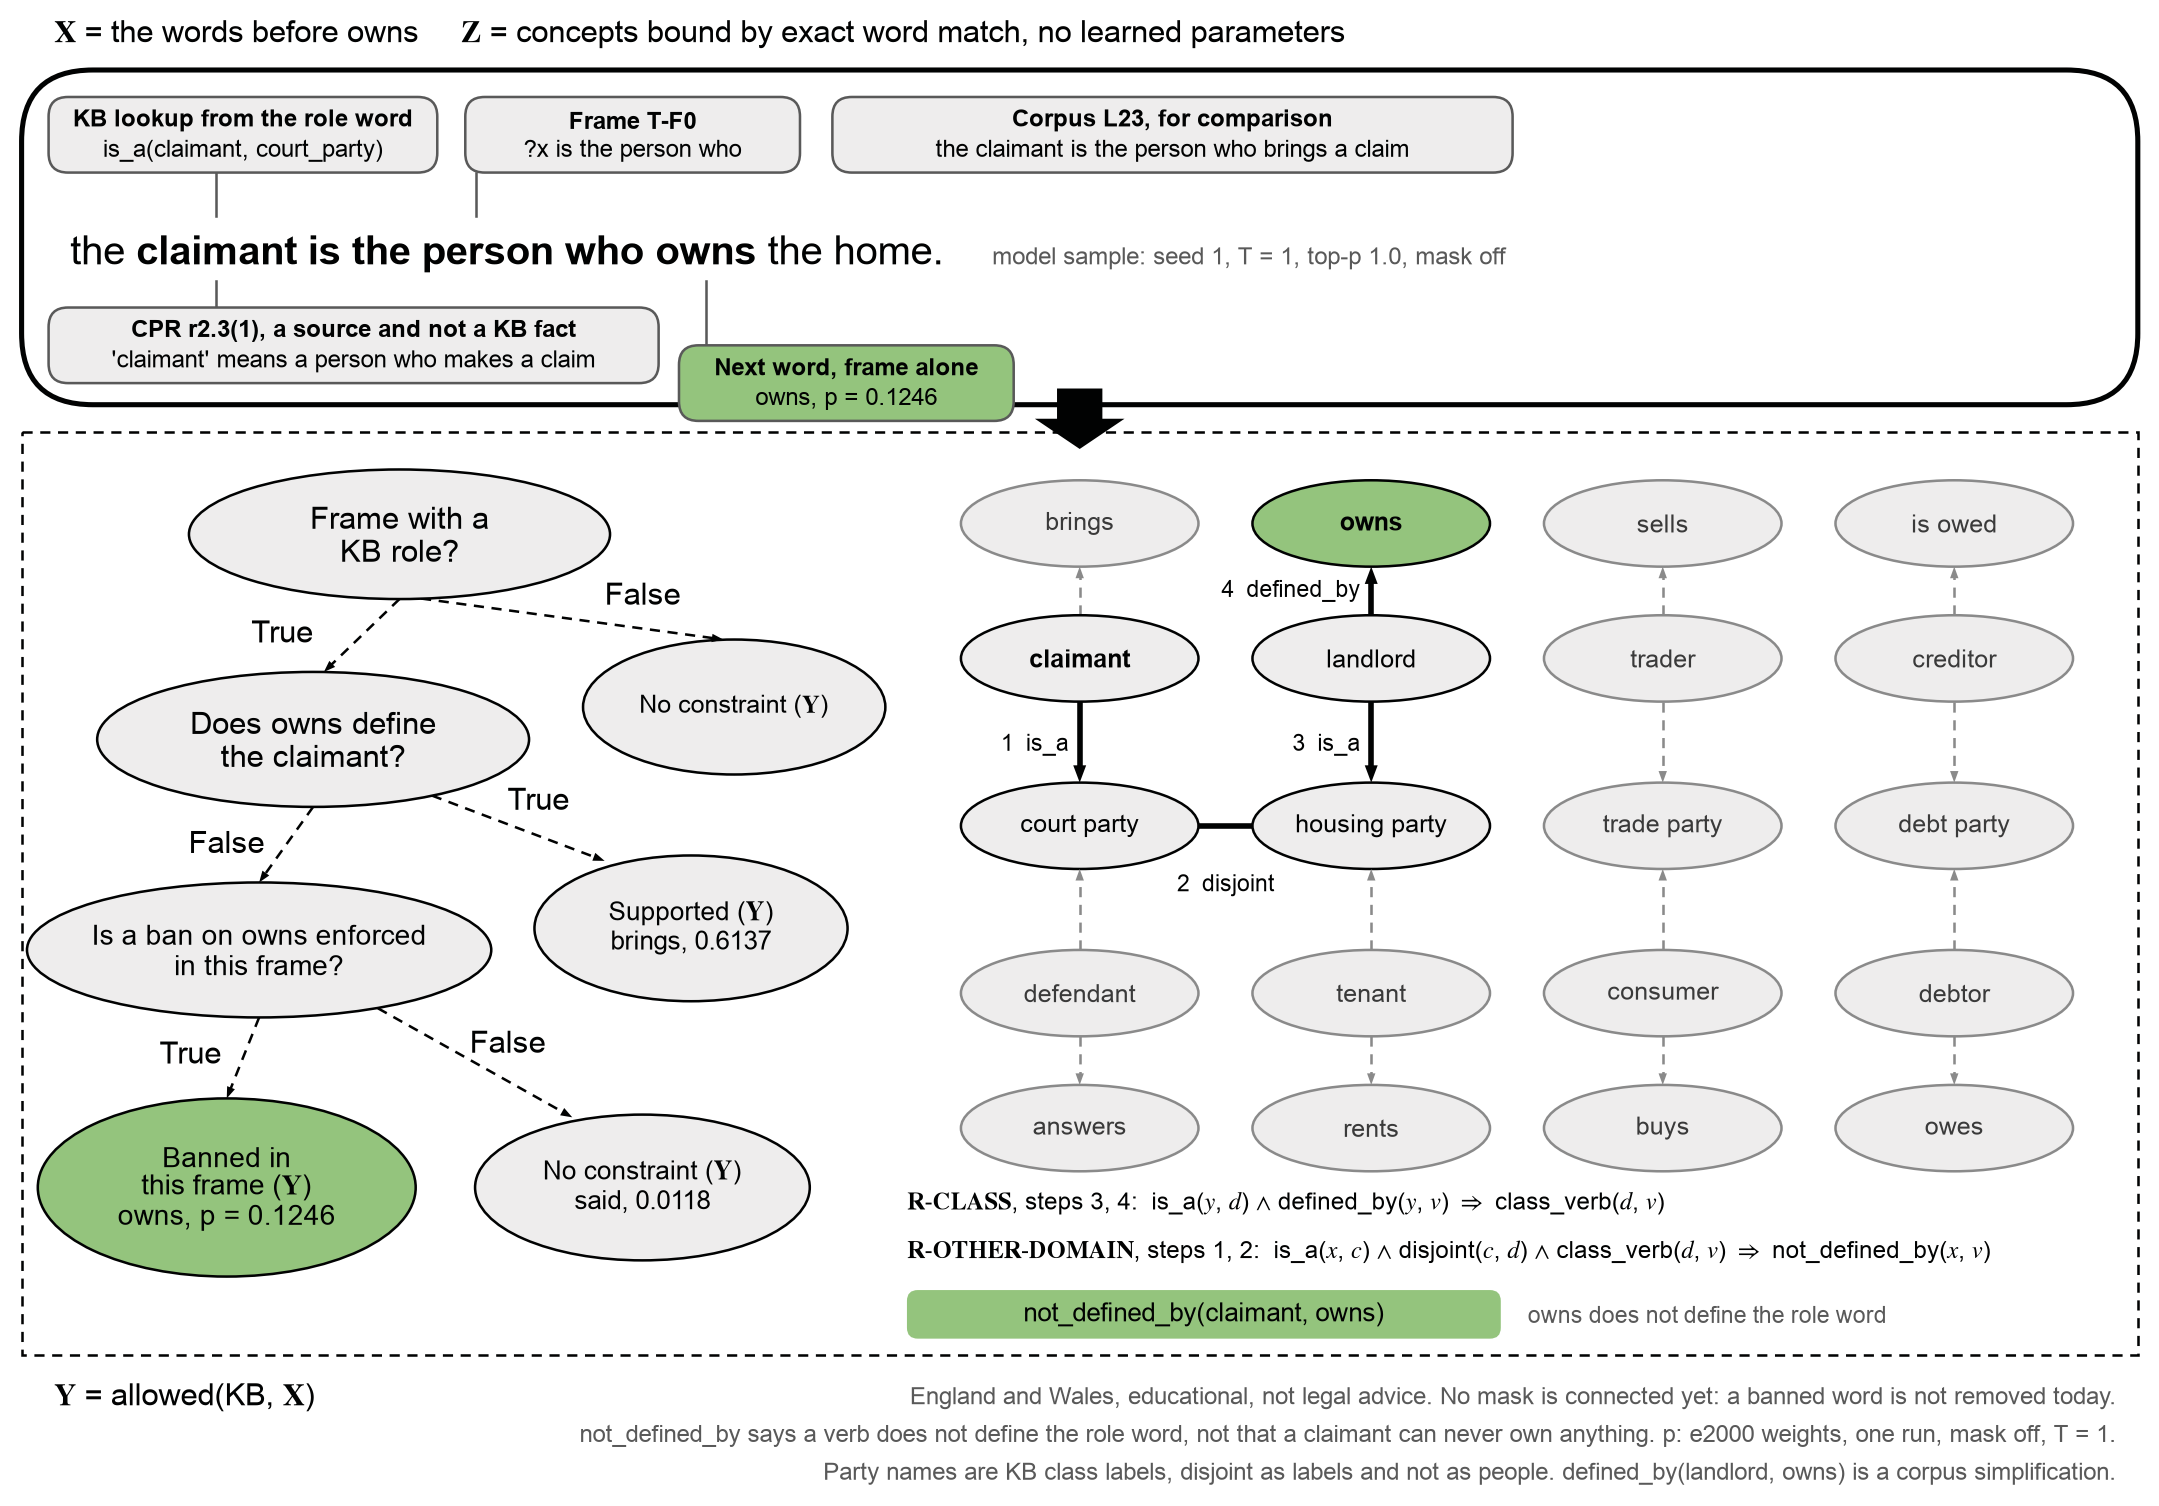
\includegraphics[width=\linewidth,trim=0 48 0 0,clip]{fig-civil-law-kb.png}\\[-2pt]
{\scriptsize\captionof{figure}{\textbf{The core logic:} one sampled sentence traced through the civil-law KB. The frame matches, two rules derive \textit{not\_defined\_by}(claimant, owns), so \emph{owns} is banned and \emph{brings} supported; $Y{=}\mathrm{allowed}(\mathrm{KB},X)$. Seed 1, $T{=}1$, mask off; educational KB, not legal advice.}\label{fig:logic}}
\end{minipage}
\end{minipage}}\vspace{2pt}}
\makeatother

\title{\LARGE\bf Neural-Symbolic NLP on a Small Transformer:\\Towards Neurosymbolic World Models for Manipulation}

\author{\applicant\thanks{Research report for EPSRC DLA project S3.5-COM-Valentino, University of Sheffield, for Dr Marco Valentino (NLP group) and Dr Amir Ghalamzan. Live demo: \url{\demourl}; try e.g.\ \texttt{300 0.8 0.9 2 40 2 42} (epochs, $T$, top-$p$, layers, tokens, $\lambda_s$, seed). Code: \url{\codeurl}.}}

\begin{document}
\maketitle
\thispagestyle{empty}
\pagestyle{empty}

%======================================================================
\section{Introduction}
Foundation models give robots broad priors but no guarantee that a step obeys a rule. Vision-language-action (VLA) policies above 90\% success on standard LIBERO fall to 0.0\% under simple perturbations~\cite{liberopro}. On Towers of Hanoi, a PDDL-based neuro-symbolic system reached 95\% against 34\% for the best fine-tuned VLA~\cite{duggan}.

The same gap appears in language at a scale small enough to inspect. In Sheth et al.~\cite{sheth2023}, an intertwined pipeline earned 70\% expert satisfaction against 47\% for a federated LLM, and process knowledge~\cite{sheth2022,roy2022} asks systems to explain themselves by the expert's guideline. On GPT-2, a pseudo-semantic loss~\cite{xu2018,ahmed2023} with word banning gave the lowest toxicity (9.20\%, against 9.80\% and 14.05\% for either alone).

This report asks: \emph{if one rule source is used in training, at decoding and to check the output, where does the constraint hold, and where does it fail?} The pairing is published~\cite{ahmed2023}; this project is a version small enough to trace every step: a from-scratch TypeScript pipeline that climbs from a rule-based chatbot to a GPT-style transformer, then adds a knowledge base (KB) used as a semantic loss, a hard logit mask and a verifier (Fig.~\ref{fig:stages}).

\begin{figure}[!htb]
\centering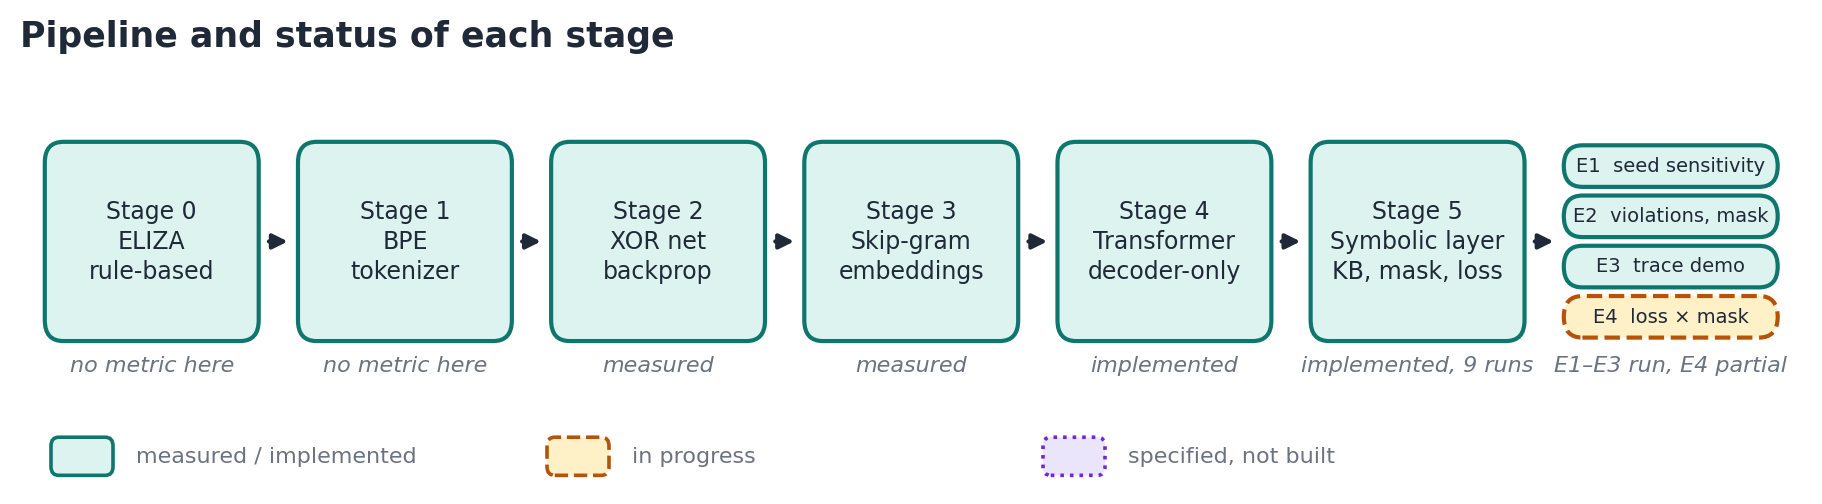
\includegraphics[width=\linewidth,trim=0 40 0 36,clip]{fig-pipeline.png}\vspace{-3pt}
\caption{Stages and status. Teal: done; amber: E4, held-out parts pending.}\label{fig:stages}
\end{figure}

%======================================================================
\section{Method}
\subsection{Baselines before the symbolic layer}
No KB, mask or semantic loss is used here. \textbf{XOR: same function, unrelated weights.} A single layer cannot learn XOR (loss 0.2845 $\to$ 0.2842); a 2$\to$4$\to$1 network can. At 5000 epochs all four seeds compute the same function with completely different hidden weights.

\textbf{Skip-gram: the civil-law vocabulary, and a wrong answer.} On England \& Wales civil-dispute text (222 definitions, 34 stories), words that share sentences end up close (Fig.~\ref{fig:sg}): buyer/customer 0.76, claimant/creditor 0.69. But none of five role analogies returns a role word (e.g.\ landlord $-$ tenant $+$ consumer gives \emph{renters}, not \emph{trader}). The model learned co-occurrence, not the relation.

\begin{figure}[!htb]
\centering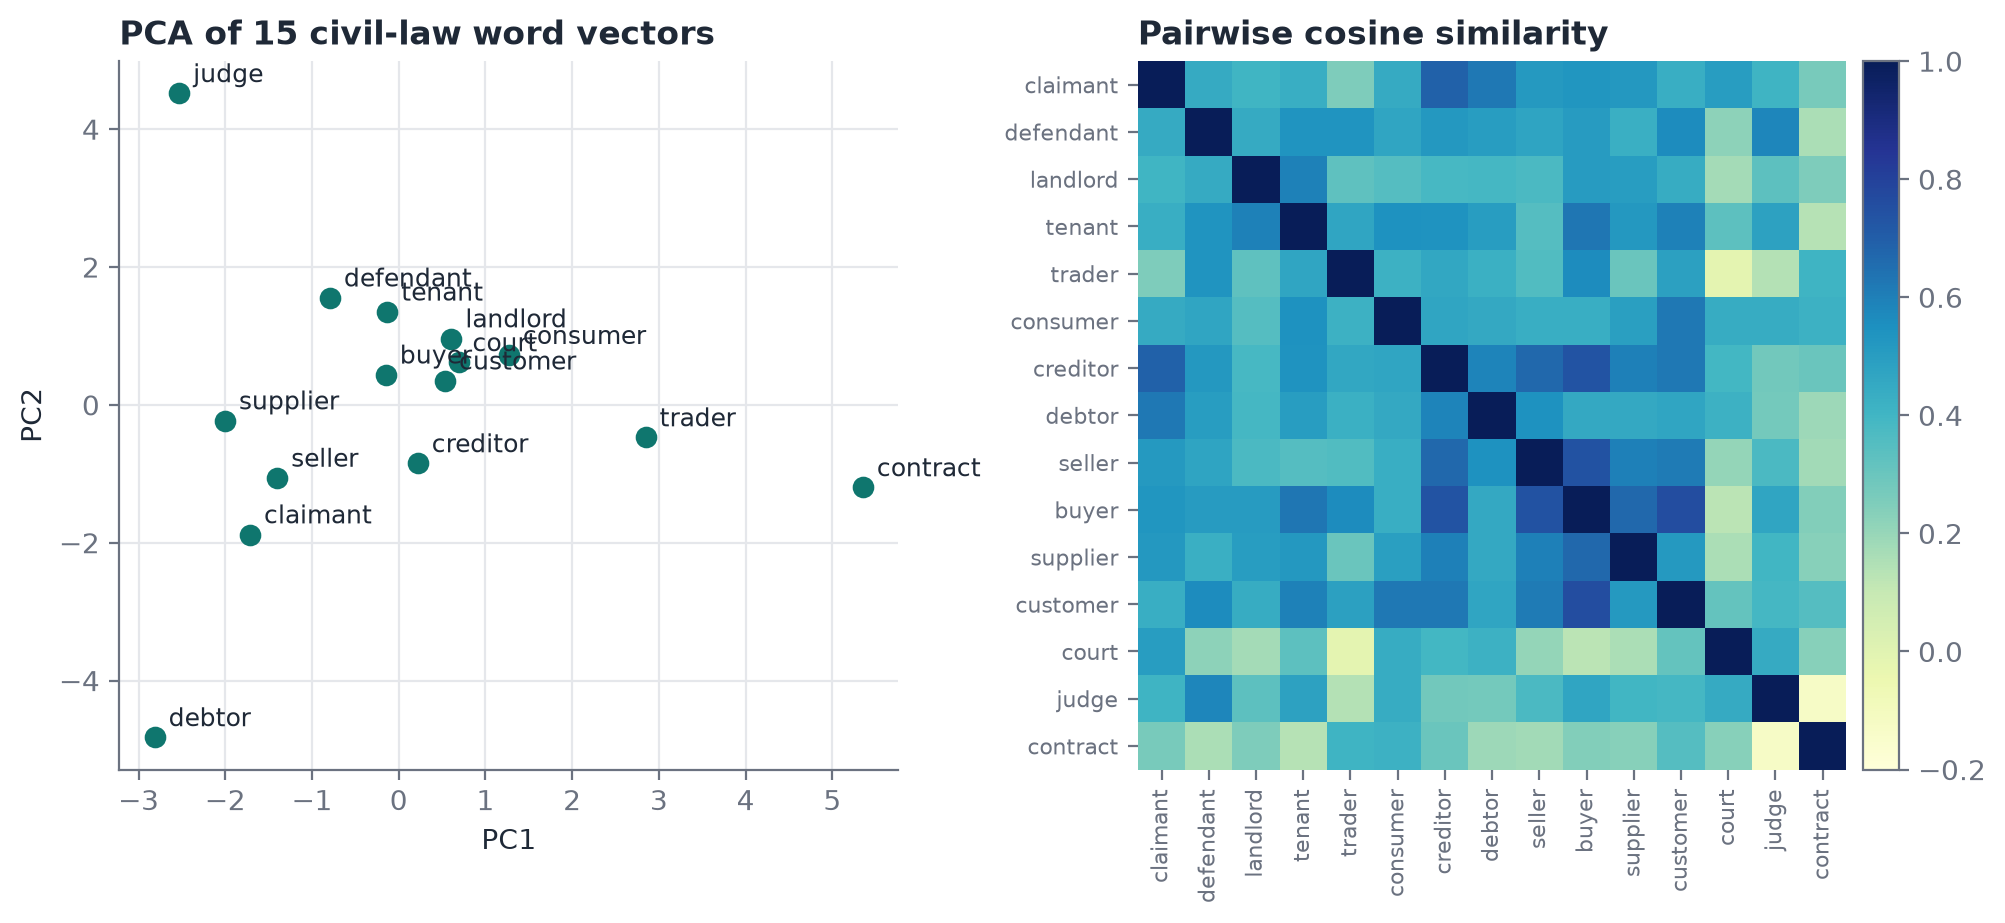
\includegraphics[width=\linewidth]{fig-skipgram-civil-law.png}\vspace{-3pt}
\caption{PCA and cosine matrix of 15 civil-law word vectors, from the saved embeddings.}\label{fig:sg}
\end{figure}

\textbf{Four seeds: the geometry agrees, the coordinates do not.} On the earlier toy corpus, the correlation of pairwise geometry across seeds is 0.977--0.984, while the same word's vectors have cosine $-0.28$ to 0.09 (Fig.~\ref{fig:seed}). The function is stable, the weights are not, and the same analogy error appears at every seed.

\begin{figure}[!htb]
\centering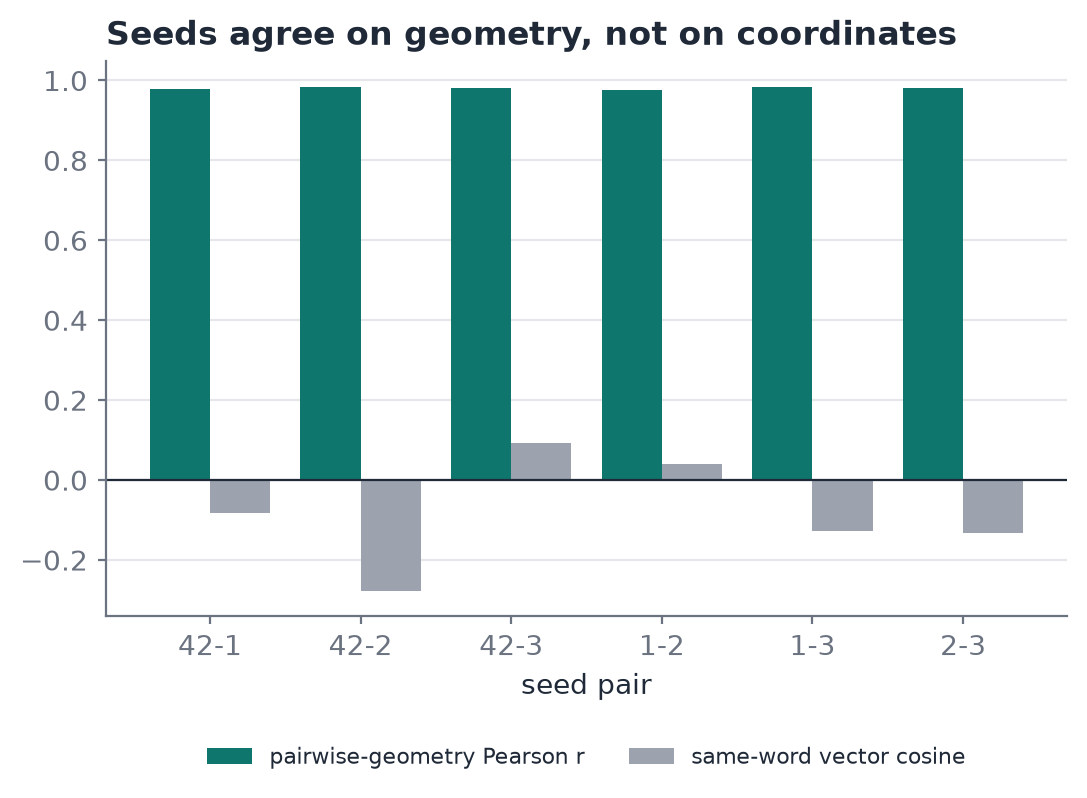
\includegraphics[width=0.8\linewidth,trim=0 0 0 22,clip]{fig-seed-agreement.png}\vspace{-3pt}
\caption{Skip-gram seed agreement, toy corpus, six seed pairs: pairwise geometry agrees, same-word vectors do not.}\label{fig:seed}
\end{figure}

\subsection{The transformer}
Each token gets a query, a key and a value; attention is $\mathrm{softmax}(QK^\top/\sqrt{d_k}+M)V$ with a causal mask $M$, so a token can only look left (Fig.~\ref{fig:qkv}). Several heads run in parallel, a feed-forward net refines each token, and blocks stack.

\begin{figure}[!htb]
\centering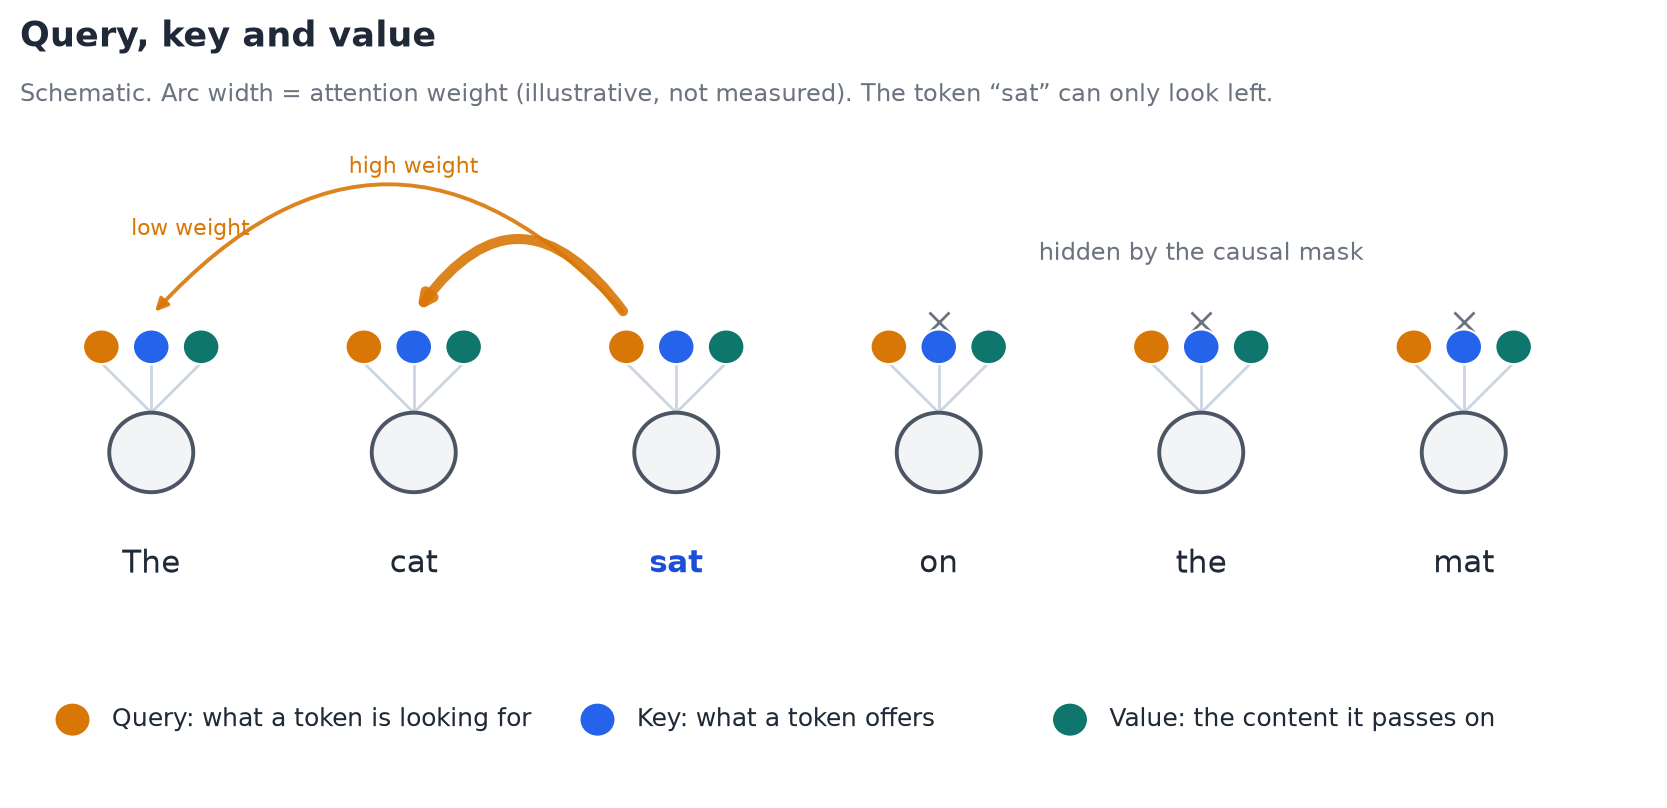
\includegraphics[width=\linewidth,trim=0 12 0 45,clip]{fig-attn-qkv.png}\vspace{-3pt}
\caption{Query, key and value. Schematic: arc width is an illustrative attention weight, not a measured one.}\label{fig:qkv}
\end{figure}

The block is pre-LayerNorm, as in GPT-2~\cite{vaswani} (Fig.~\ref{fig:block}): $x'=x+\mathrm{MHA}(\mathrm{LN}_1(x))$, $x''=x'+\mathrm{FFN}(\mathrm{LN}_2(x'))$. Forward, backward, Adam and top-$p$ sampling are written by hand and pass five gates, including a finite-difference gradient check. The model has 2 layers, $d{=}32$, 2 heads, feed-forward width 128 and context 32: 87,401 parameters with the 937-token whole-word BPE vocabulary.

\begin{figure}[!htb]
\centering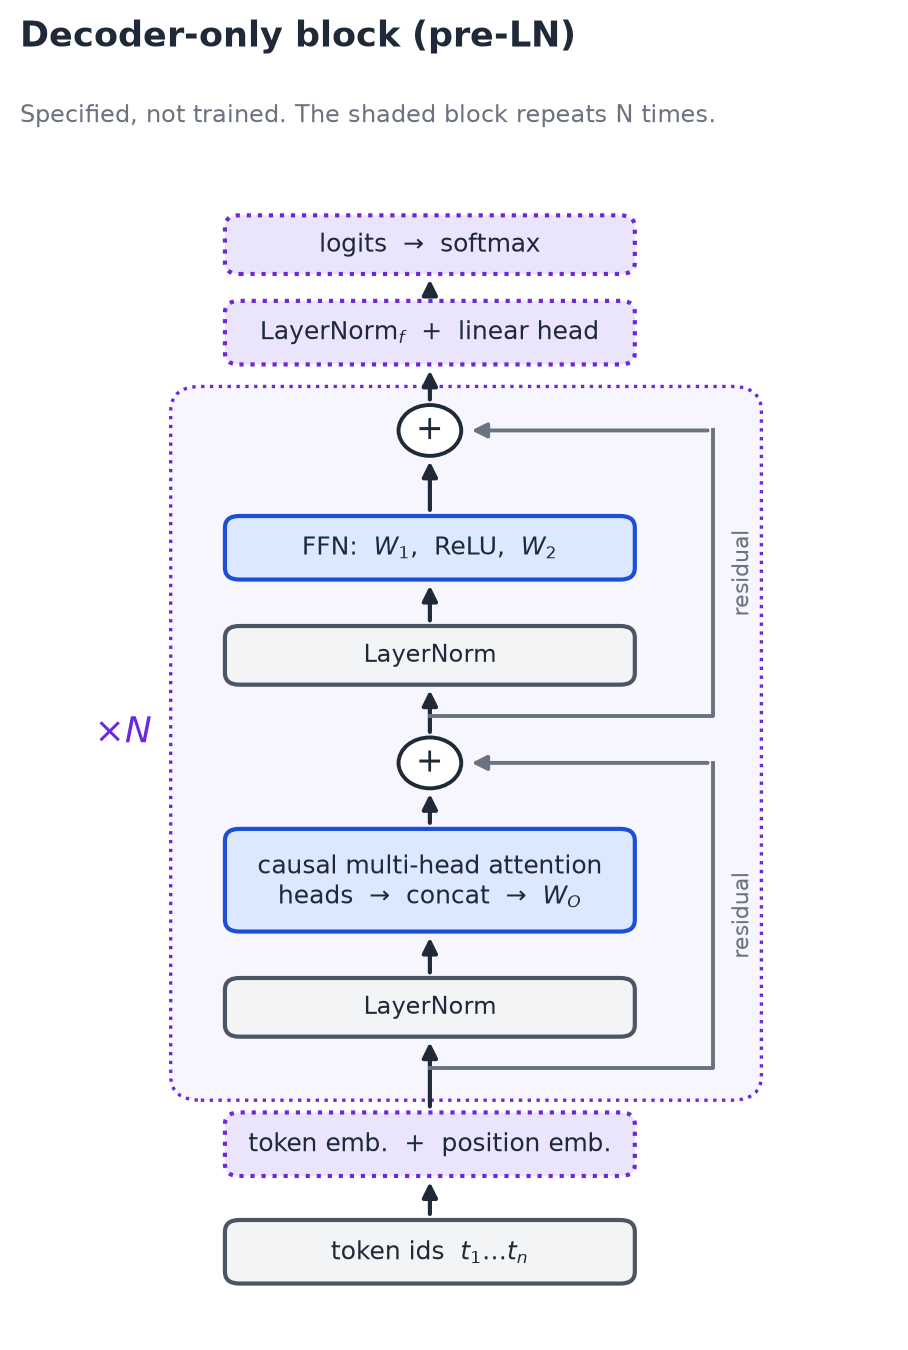
\includegraphics[width=0.5\linewidth,trim=0 18 0 66,clip]{fig-transformer-block.png}\vspace{-3pt}
\caption{The decoder-only block (pre-LN), implemented in \texttt{transformer.ts}. The shaded block repeats $N$ times.}\label{fig:block}
\end{figure}

\textbf{The reasoning gap.} The objective has no notion of truth: it rewards sounding like the corpus. Equal behaviour comes from unrelated weights, so attention maps show where the model looked, not a justification. The semantic loss has limits too: 69.89\% of test predictions satisfied the constraint on grid paths in~\cite{xu2018}, and a wrong rule is trained in.

\subsection{Mechanisms and the taxonomy}
In the terms of Sheth et al.~\cite{sheth2023}, \emph{lowering} compresses knowledge into the network and \emph{lifting} lifts its output into symbols (Fig.~\ref{fig:tax}). In our mapping, the mask and soft bias are 1a-style lowering by analogy, the verifier and reasoning trace are decoupled lifting (2a), and the semantic loss moves toward intertwined integration (2b).

\begin{figure}[!htb]
\centering\includegraphics[page=3,trim=60 123 47 383,clip,width=\linewidth]{../paper/Neurosymbolic_Artificial_Intelligence_Why_What_and_How.pdf}\vspace{-3pt}
\caption{Taxonomy of neurosymbolic AI methods, reproduced from~\cite{sheth2023}, Fig.~1; L/M/H are its authors' ratings. Where this work sits is our mapping (text).}\label{fig:tax}
\end{figure}

At decoding, the KB feeds a logits processor between the transformer and sampling, which records a reasoning trace (rules fired, mass moved), and a verifier checks the finished text (Fig.~\ref{fig:flow}).

\par\smallskip\noindent\begin{minipage}{\linewidth}
\centering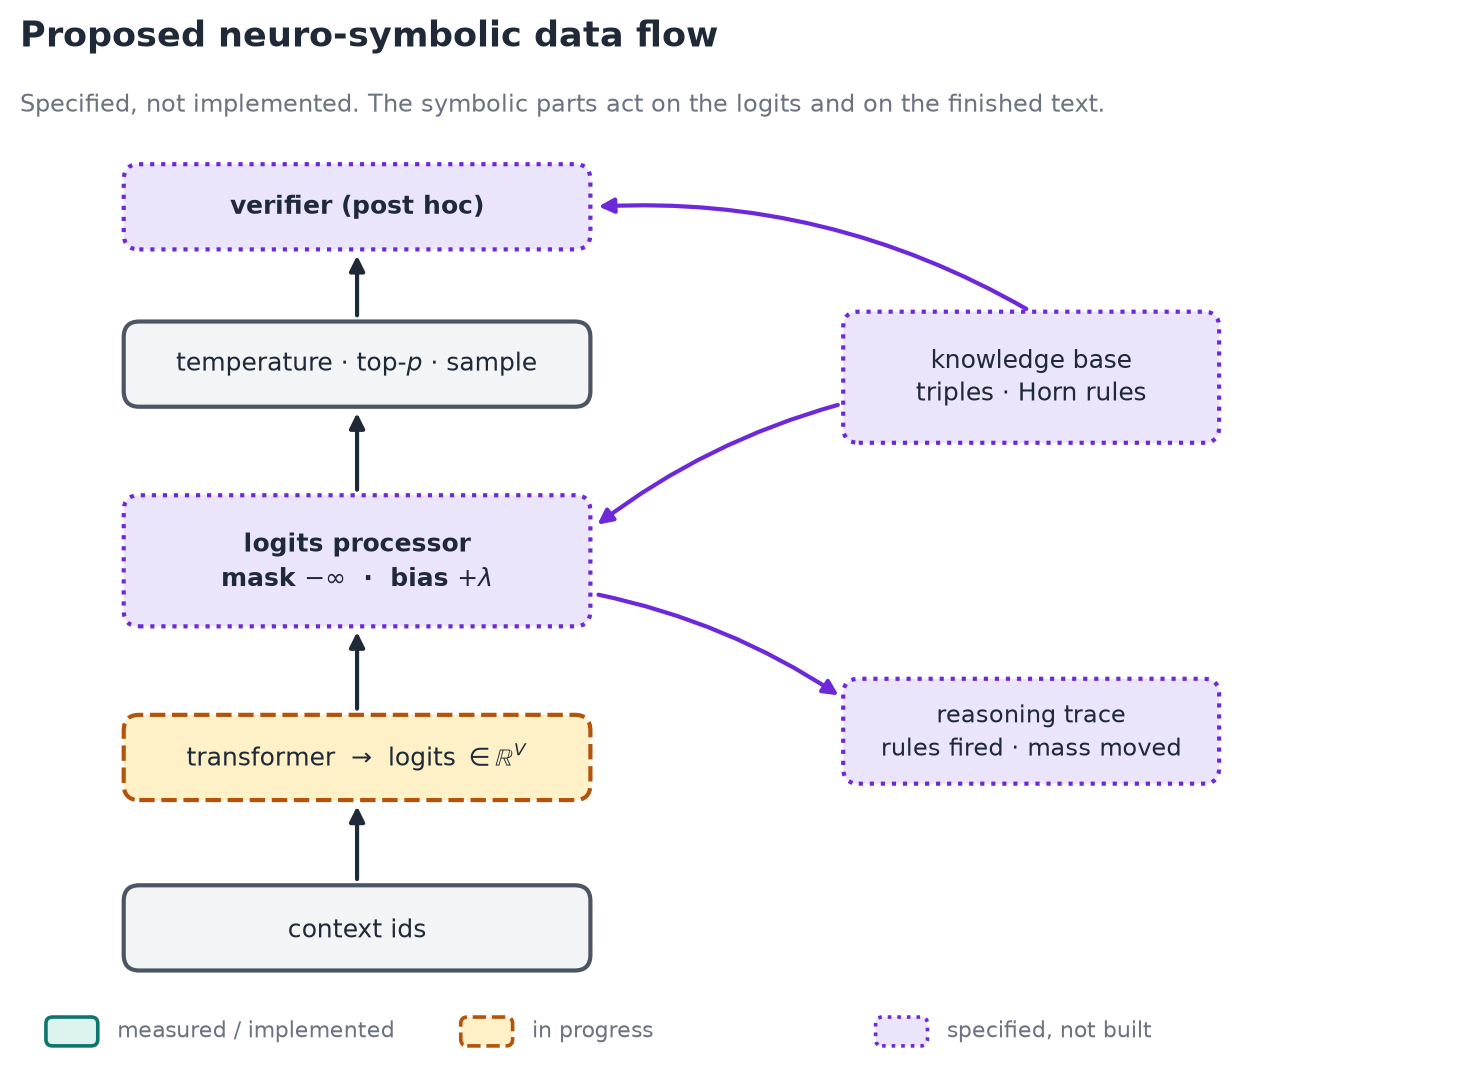
\includegraphics[width=0.72\linewidth,trim=0 0 0 46,clip]{fig-neurosymbolic-flow.png}\vspace{-3pt}
\captionof{figure}{Neuro-symbolic data flow at decoding. \emph{Status note:} drawn before the symbolic layer was built; the parts marked ``specified, not built'' are now implemented.}\label{fig:flow}
\end{minipage}\par\smallskip

\begin{figure*}[!t]
\centering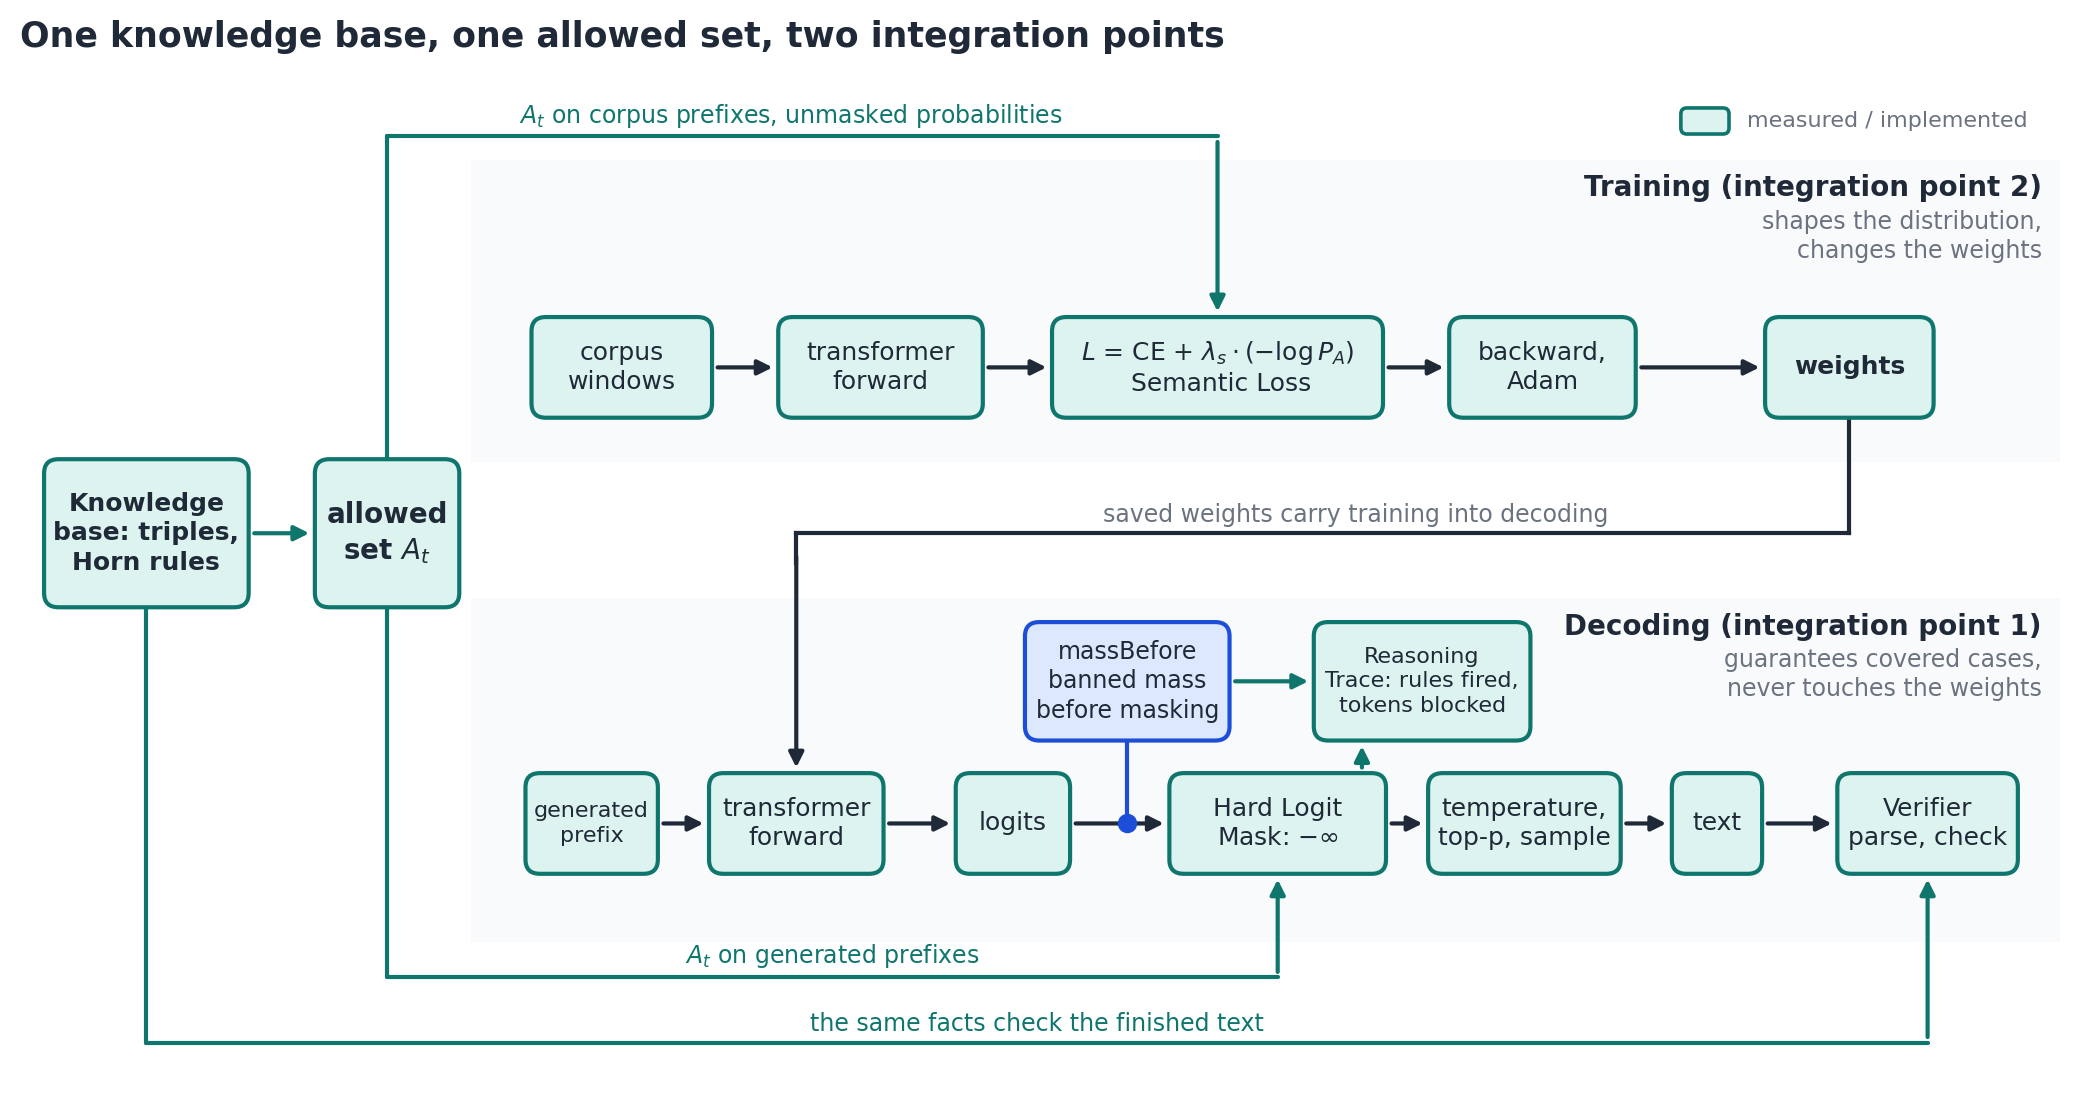
\includegraphics[width=0.68\textwidth,trim=0 0 0 22,clip]{fig-design-pipeline.png}\vspace{-3pt}
\caption{One KB gives one allowed set, used by the semantic loss in training and by the hard mask at decoding; \textit{massBefore} marks where the trained model meets the mask.}\label{fig:pipe}
\end{figure*}

\subsection{Pre-training: the baseline before the symbolic layer}
The CE-only transformer trained 2000 epochs (seed 42) on all of the text. Its loss fell from 6.868 ($\approx\ln 937$) to 0.2489, but \textbf{this loss shows memorisation}: from epoch 1510 on, 100\% of generated tokens sit inside runs of 8 or more tokens copied from the training text. Earlier, fluent samples stated definitions the corpus does not contain: ``the claimant is the person who \emph{owns} the home'' (the corpus says \emph{brings a claim}). Low loss is not correctness.

\subsection{One knowledge base, two integration points}
The two designs are not alternatives. A KB of triples plus Horn rules gives one allowed set $A_t$ per position, and that set is used twice (Fig.~\ref{fig:pipe}): training shapes the distribution, and decoding guarantees the covered cases, as in~\cite{ahmed2023}.

The KB covers definitions in the corpus, e.g.\ with $c$ the claimant and $d$ the defendant, $\mathit{counterpart}(c,d)\wedge\mathit{defined\_by}(d,\mathrm{answers})\Rightarrow\mathit{not\_defined\_by}(c,\mathrm{answers})$. Forward chaining closes it once; a trigger turns a derived fact into banned token IDs when the context ends in a frame such as ``the claimant is the person who'', and every ban prints as a proof (Fig.~\ref{fig:logic}: \emph{owns}, $p{=}0.1246$, is banned).

\textbf{Method 1: hard logit mask.} Banned logits are set to $-\infty$ before temperature and top-$p$. This guarantees zero mass on covered banned tokens, but only as far as rules and triggers reach, and a wrong rule is enforced absolutely. It does not change the weights.

\textbf{Method 2: semantic loss.} $\mathcal{L}=\mathrm{CE}+\lambda_s(-\log P_A)$, with $P_A$ the mass on allowed tokens~\cite{xu2018,ahmed2023}. It depends on $P_A$ alone, so it cannot see the choice among allowed tokens; it acts only where a rule fires (86 of 85,984 positions); and it is a soft penalty with no test-time guarantee.

\textbf{Why the loss needs the mask.} No finite $\lambda_s$ removes all banned mass, so a correct rule still needs the mask; the loss shows in \textit{massBefore} and in violations with the mask off.

\textbf{Lifting.} A verifier labels each generated claim \emph{supported}, \emph{contradicted} or \emph{unknown}. A probe reads confident predictions as candidate facts (\emph{confirmed}, \emph{conflict}, \emph{novel}), reported but never added to the KB. \textbf{Two trainers.} The baseline and the neural-symbolic model share corpus, tokenizer, model code and hyperparameters; only the loss differs, and $\lambda_s{=}0$ at seed 42 reproduces the baseline's weights exactly.

\subsection{Protocol}
Prompts are every role in every definition frame ($8\times3$): 8 occur in the training text, and 16 put a role in a frame it never appears in (``the claimant is a business that''), the only held-out data. Each is sampled at seeds 0--49 for 20 tokens at two settings, mask off and on. A rule is violated when its banned word's mean $p$ at its trigger is ${\ge}0.02$. All runs train 2000 epochs: one at $\lambda_s{=}50$ against the CE-only baseline (seed 42), and eight at $\lambda_s\in\{0,2\}\times$ seeds 42, 1, 2, 3.

%======================================================================
\section{Results}
\subsection{One full-length run: $\lambda_s{=}50$ against CE only}
At the 86 positions where a rule fires (Table~\ref{tab:l50}), CE only violates a rule at 1846 of 2001 epochs; the constrained model at 175, none after epoch 1746. The banned mass is lower at every logged epoch, and the semantic loss 73 times lower at epoch 2000; both curves rise and fall, peaking at 4.73e-4 (epoch 689) without the term and 2.26e-5 (epoch 585) with it (Fig.~\ref{fig:l50}). Up to about epoch 600 the term also slows the allowed words; by epoch 1000 it is ahead. Training loss costs a little (0.2524 against 0.2489, on all text).

\begin{figure}[!htb]
\centering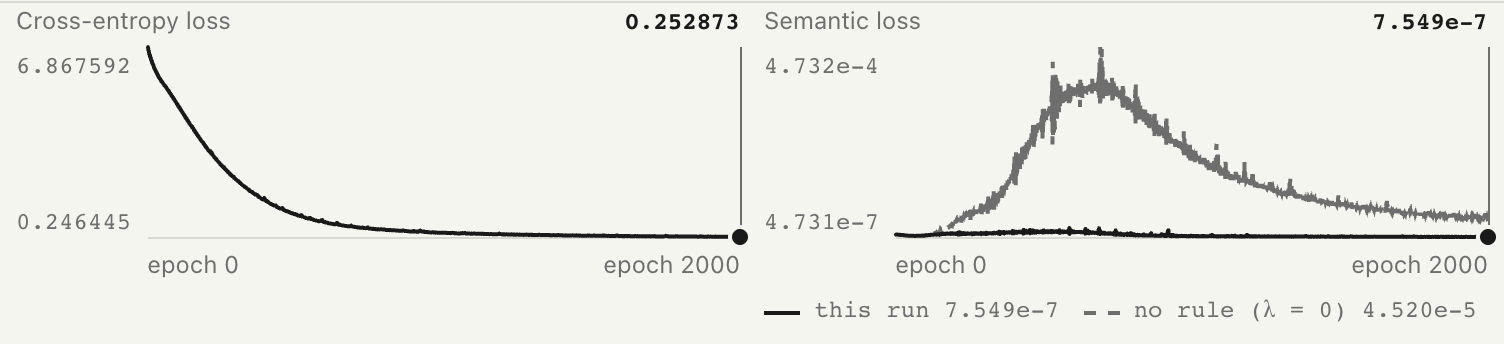
\includegraphics[width=\linewidth]{ns-l50-vs-l0-e2000-loss.png}\vspace{-3pt}
\caption{The $\lambda_s{=}50$ run in the live demo: cross-entropy (left) and semantic loss (right) by epoch, $\lambda_s{=}0$ control dashed; values as logged in training (Table~\ref{tab:l50} reads the saved weights).}\label{fig:l50}
\end{figure}

\begin{table}[!htb]
\caption{Epoch 2000, seed 42, the 86 constrained training positions.}\label{tab:l50}
\centering\footnotesize\setlength{\tabcolsep}{4pt}
\begin{tabular}{@{}lrr@{}}
\toprule
Measure & CE only & CE + sem.\ loss\\
\midrule
Semantic loss & 4.58e-5 & 6.26e-7\\
Banned mass & 0.0419 & 0.0006\\
$p$(next corpus word) & 0.946 & 0.978\\
$p$(role's own verb) & 0.809 & 0.841\\
Rules violated (of 48) & 7 & 0\\
\bottomrule
\end{tabular}
\end{table}

\subsection{E2 and E3 at one training seed}
With the mask on, 0 of 5,885 claims contradict the KB at this seed. With the mask off, the $\lambda_s{=}50$ model made no contradicted claim in 1,173 on the 8 training-text prompts (CE only: 1.2\% at $T{=}0.8$, 4.8\% at $T{=}1$). On the 16 untrained prompts it still contradicts the KB in 35--36\% of claims (CE only 41--43\%), mostly with the verb of the one role trained in that frame (315 of 430 are ``sells'' after ``is a business that''): the frame, not the role, appears to drive it (untested). In E3, \textit{massBefore} on banned verbs was 0.3252 (CE) against 0.0026.

\subsection{E1 and E4: four training seeds}
Table~\ref{tab:e4} compares $\lambda_s{=}2$ with 0. A paired sign-flip test over 4 seeds cannot go below $p{=}0.125$, so ``at every seed'' is not a significance claim.

\begin{table}[!htb]
\caption{Seeds 42, 1, 2, 3, $\lambda_s{=}0$ vs 2, mask off; ranges over seeds or seed pairs.}\label{tab:e4}
\centering\footnotesize\setlength{\tabcolsep}{3pt}
\begin{tabular}{@{}lrr@{}}
\toprule
Measure & $\lambda_s{=}0$ & $\lambda_s{=}2$\\
\midrule
Banned mass, 86 constrained pos. & 0.024--0.049 & 0.008--0.016\\
Banned mass, 16 untrained prompts & 0.45--0.73 & 0.43--0.71\\
Contradicted, untrained, $T{=}0.8$ & 35.4--47.9\% & 31.3--45.7\%\\
JS of $(P_A,1{-}P_A)$, mean & 7.5e-3 & 2.5e-3\\
JS of $q_A$ (among allowed), mean & 0.0153 & 0.0149\\
Perplexity, no rule fires (train) & 1.266--1.283 & 1.264--1.281\\
\bottomrule
\end{tabular}
\end{table}

\textbf{Seeds (E1).} At $\lambda_s{=}0$, loss is similar but weights nearly unrelated; seeds agree on the next word at every training-text prompt, but at only 50--69\% of held-out ones.

\textbf{Semantic loss (E4).} Banned mass at constrained positions is 2.6--4.3$\times$ lower at every seed; seeds disagree three times less on mass to allowed words, not \emph{among} them, as Method 2 predicts. On untrained prompts the effect is small.

\textbf{Mask coverage.} With the mask on, 514 of 23,664 claims still contradict the KB, all ``that \emph{owed} money'', which the mask bans only after ``is'': a coverage gap, not a model property.

%======================================================================
\section{Conclusion}
\textbf{Where the constraint is trained, it holds}, at a small cost in training loss. \textbf{Beyond it, the rule does not transfer}: on unseen frames the model follows the frame, not the KB. \textbf{A guarantee covers only what its rules cover}, as the ``owed'' gap shows. Limits: one small model, a hand-written KB, four seeds, no held-out text.

\textbf{Towards neurosymbolic world models.} Tokens become actions and states, and the allowed set becomes PDDL preconditions, effects and contact constraints such as slip bounds; the loss trains the world model, the mask rejects actions, and the verifier triggers recovery. \emph{O1 (Years 1--2):} a multimodal model proposes PDDL action models under training and decoding constraints~\cite{xu2018,ahmed2023}, with semantic faithfulness checked by prover-based verification~\cite{quan2024,quan2025} (GPT-4o's PDDL was 96.1\% parseable but 24.8\% correct~\cite{planetarium}); it also tests whether world models follow plausibility over validity, like the frame effect above, and whether steering~\cite{valentino2026,kim2025} reduces it. \emph{O2 (Years 2--3):} a slow symbolic layer sets subgoals and constraints; a fast controller rolls out an action-conditioned tactile model~\cite{mandil,nazari2022} and checks constraints on predicted states, so a predicted violation triggers replanning before failure, compared with post-failure recovery~\cite{reflect}, against VLA and LLM-planner baselines~\cite{liberopro,duggan}. The main risk is a wrong rule entering training and decoding at once, so every rule stays traceable to a proof.

\textbf{Any LLM.} As a \emph{federated pipeline}~\cite{sheth2023}, the access points of Fig.~\ref{fig:pipe} become API levels: weights take the loss, logits the mask, text the verifier~\cite{quan2024,quan2025,llmmodulo}. Designed, not built.

\begin{thebibliography}{99}
\scriptsize
\setlength{\itemsep}{0pt}
\bibitem{liberopro} X.~Zhou \emph{et al.}, ``LIBERO-PRO: Towards robust and fair evaluation of vision-language-action models beyond memorization,'' arXiv:2510.03827, 2025.
\bibitem{duggan} T.~Duggan \emph{et al.}, ``The price is not right: Neuro-symbolic methods outperform VLAs on structured long-horizon manipulation tasks,'' in \emph{Proc. ICRA}, 2026.
\bibitem{sheth2023} A.~Sheth, K.~Roy, and M.~Gaur, ``Neurosymbolic artificial intelligence (why, what, and how),'' \emph{IEEE Intell. Syst.}, vol.~38, no.~3, pp.~56--62, 2023.
\bibitem{sheth2022} A.~Sheth, M.~Gaur, K.~Roy, R.~Venkataraman, and V.~Khandelwal, ``Process knowledge-infused AI: Towards user-level explainability, interpretability, and safety,'' arXiv:2206.13349, 2022.
\bibitem{roy2022} K.~Roy, M.~Gaur, Q.~Zhang, and A.~Sheth, ``Process knowledge-infused learning for suicidality assessment on social media,'' arXiv:2204.12560, 2022.
\bibitem{xu2018} J.~Xu, Z.~Zhang, T.~Friedman, Y.~Liang, and G.~Van den Broeck, ``A semantic loss function for deep learning with symbolic knowledge,'' in \emph{Proc. ICML}, 2018.
\bibitem{ahmed2023} K.~Ahmed, K.-W.~Chang, and G.~Van den Broeck, ``A pseudo-semantic loss for autoregressive models with logical constraints,'' in \emph{Proc. NeurIPS}, 2023.
\bibitem{vaswani} A.~Vaswani \emph{et al.}, ``Attention is all you need,'' in \emph{Proc. NeurIPS}, 2017.
\bibitem{quan2024} X.~Quan, M.~Valentino, L.~A.~Dennis, and A.~Freitas, ``Verification and refinement of natural language explanations through LLM-symbolic theorem proving,'' in \emph{Proc. EMNLP}, 2024.
\bibitem{quan2025} X.~Quan, M.~Valentino, L.~A.~Dennis, and A.~Freitas, ``Faithful and robust LLM-driven theorem proving for NLI explanations,'' in \emph{Proc. ACL}, 2025.
\bibitem{llmmodulo} S.~Kambhampati \emph{et al.}, ``LLMs can't plan, but can help planning in LLM-Modulo frameworks,'' in \emph{Proc. ICML}, 2024.
\bibitem{planetarium} M.~Zuo \emph{et al.}, ``Planetarium: A rigorous benchmark for translating text to structured planning languages,'' in \emph{Proc. NAACL}, 2025.
\bibitem{valentino2026} M.~Valentino, G.~Kim, D.~Dalal, Z.~Zhao, and A.~Freitas, ``Mitigating content effects on reasoning in language models through fine-grained activation steering,'' in \emph{Proc. AAAI}, 2026.
\bibitem{kim2025} G.~Kim, M.~Valentino, and A.~Freitas, ``Reasoning circuits in language models: A mechanistic interpretation of syllogistic inference,'' in \emph{Findings of ACL}, 2025.
\bibitem{mandil} W.~Mandil, K.~Nazari, and A.~Ghalamzan~E, ``Action conditioned tactile prediction: A case study on slip prediction,'' arXiv:2205.09430, 2022.
\bibitem{nazari2022} K.~Nazari, W.~Mandil, and A.~Ghalamzan~E, ``Proactive slip control by learned slip model and trajectory adaptation,'' arXiv:2209.06019, 2022.
\bibitem{reflect} Z.~Liu, A.~Bahety, and S.~Song, ``REFLECT: Summarizing robot experiences for failure explanation and correction,'' in \emph{Proc. CoRL}, 2023.
\end{thebibliography}

\end{document}
